
\subsection{Higher moments closure : Stresslet ? ? }


\begin{equation}
    \ddt \mathcal{P}_\alpha
    = \int_{\Omega_\alpha} \left(
        \rho_2  \textbf{w}_2 \textbf{w}_2 
        + \textbf{r} \div \mathbf{T}_2
    \right) d\Omega
\end{equation}
\begin{equation}
    \ddt \mathcal{P}_\alpha
    = \int_{\Omega_\alpha} \left(
        \rho_2  \textbf{w}_2 \textbf{w}_2 
        + \mathbf{T}_2
    \right) d\Omega
+ \int_{\Sigma}\textbf{rT}_2 \cdot \textbf{n}_2 d\Sigma
\end{equation}
surface jump condition : 
\begin{equation}
    - \int_{\Sigma_\alpha} 
    \sigma \textbf{I}_{||}
d\Sigma
= \int_{\Sigma}\textbf{rT}_1 \cdot \textbf{n}_1 d\Sigma
+ \int_{\Sigma}\textbf{rT}_2 \cdot \textbf{n}_2 d\Sigma
\end{equation}
\begin{equation}
    \ddt \mathcal{P}_\alpha
    = \int_{\Omega_\alpha} \left(
        \rho_2  \textbf{w}_2 \textbf{w}_2 
        - \mathbf{T}_2
    \right) d\Omega
    - \int_{\Sigma_\alpha} 
        \sigma \textbf{I}_{||}
    d\Sigma
    + \int_{\Sigma}\textbf{rT}_1 \cdot \textbf{n}_2 d\Sigma
\end{equation}
\begin{figure}[h!]
    \centering
    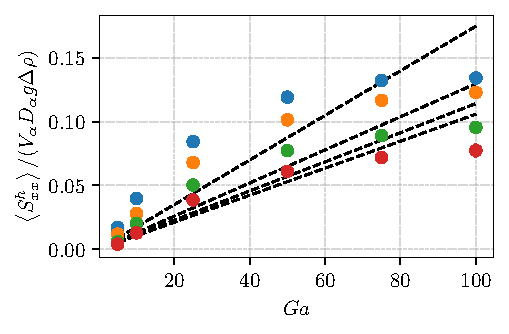
\includegraphics[height=0.3\textwidth]{image/HOMOGENEOUS/fPA/Sxx.pdf}
    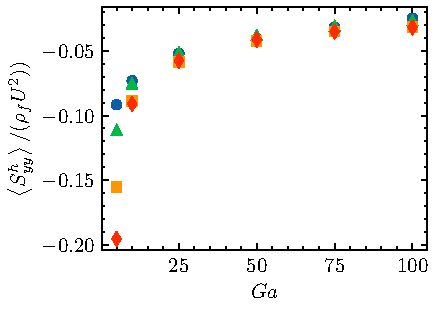
\includegraphics[height=0.3\textwidth]{image/HOMOGENEOUS/fPA/Syy.pdf}
\end{figure}
\begin{equation}
    \int_{\Sigma}\textbf{r}_1 (\textbf{T}_1  -  \oneavg{\textbf{T}_1}) \cdot \textbf{n}_2 d\Sigma
    = \int_{\Omega_\alpha} \left(
        \mathbf{T}_2
        - \rho_2  \textbf{w}_2 \textbf{w}_2 
    \right) d\Omega
     + \int_{\Sigma_\alpha} 
     \sigma \textbf{I}_{||}
    d\Sigma
    + \ddt \mathcal{P}_\alpha
    -\int_{\Sigma}\textbf{r}_1   \oneavg{\textbf{T}_1} \cdot \textbf{n}_2 d\Sigma
\end{equation}
Assuming that $\textbf{T}_k = - p_k \textbf{I} + \mu_k \mathbb{S}_k  = -p_k \textbf{I} + \mu_k (\grad \textbf{u}_k + \grad \textbf{u}_k^T )$ 
\begin{multline}
    \int_{\Sigma}\textbf{r}_1 (\textbf{T}_1  -  \oneavg{\textbf{T}_1}) \cdot \textbf{n}_2 d\Sigma
    \\= \dot{ \mathcal{P}_\alpha}
    + \int_{\Omega_\alpha} \left(
        \mu_2\mathbb{S}_2
        - \rho_2  \textbf{w}_2 \textbf{w}_2 
    \right) d\Omega
     + \int_{\Sigma_\alpha} 
     \sigma \textbf{I}_{||}
    d\Sigma
    - \textbf{I} \int_{\Omega_\alpha} p_2 d\Omega
    + v_\alpha \oneavg{p}
    - \mu_1 v_\alpha \oneavg{\mathbb S}
\end{multline}
\begin{multline}
    \int_{\Sigma}\textbf{r}_1 (\textbf{T}_1  -  \oneavg{\textbf{T}_1}) \cdot \textbf{n}_2 d\Sigma
    \\= \dot{ \mathcal{P}_\alpha}
    + \int_{\Omega_\alpha} \left(
        \mu_2\mathbb{S}_2
        - \rho_2  \textbf{w}_2 \textbf{w}_2 
    \right) d\Omega
     + \int_{\Sigma_\alpha} 
     \sigma \textbf{I}_{||}
    d\Sigma
    - \textbf{I} \int_{\Omega_\alpha} p_2 d\Omega
    + v_\alpha \oneavg{p}
    - \mu_1 v_\alpha \oneavg{\mathbb S}
\end{multline}
Keeping only  the deviatoric part of the equations
\begin{equation}
    \textbf{S}_\alpha
    = \dot{ \mathcal{P}_\alpha}
    + \int_{\Omega_\alpha} \left(
        \mu_2\mathbb{S}_2
        - \rho_2  \textbf{w}_2 \textbf{w}_2 + w^2_2/3
    \right) d\Omega
     + \int_{\Sigma_\alpha} 
     \sigma \textbf{I}_{||}^{dev}
    d\Sigma
    - \mu_1 v_\alpha \oneavg{\mathbb S}
\end{equation}
For an almost spherical drop in a stokes regime: 
\begin{equation}
    \textbf{S}_\alpha
    = 
    \int_{\Omega_\alpha} \left(
        \mu_2\mathbb{S}_2
    \right) d\Omega
    - \mu_1 v_\alpha \oneavg{\mathbb S}
\end{equation}
 
The original formulas stipulate that :

\todo{This formulation must be chnaged look at \citet[chap 5]{pozrikidis1992boundary}}
\begin{align}
    \label{eq:M_decomposition}
    S^\alpha_{ij} 
    &= \frac{1}{2}  \int_{\Sigma_\alpha} \left[
        r_i(T_{jk}n_k)
        + (T_{ik}n_k)r_j
        \right]d\Sigma
        - \frac{\delta_{ij}}{3}\int_{\Sigma_\alpha} \left[
            r_l(T_{lk}n_k)
    \right]d\Sigma
    -\mu_1 \int_{\Sigma_{\alpha}}
    (u_in_j^2 + u_jn_i^2)d\Sigma
    \\
    T^\alpha_{ij}
    &= \frac{1}{2}  \int_{\Sigma_\alpha} \left[
        r_i(T_{jk}n_k)
        - (T_{ik}n_k)r_j
    \right]d\Sigma \nonumber
\end{align}

Inter changing the sens of the normal vector we can rewrite the last term of \ref{eq:M_decomposition} such as :
\begin{align}
    - \mu_1 \int_{\Sigma_{\alpha}}
    (u_in_j + u_jn_i)d\Sigma
    = 
    + \mu_1 \int_{\Sigma_{\alpha}}
    (u_i n^1_j + u_jn^1_i)d\Sigma
\end{align}
Using Gauss divergence theorem 
\begin{align}
    - \mu_1 \int_{\Sigma_{\alpha}}
    (u_in_j + u_jn_i)d\Sigma
    = 
    \mu_1 \int_{\Omega_1}
    (\grad u_i + \grad u_j )d\Omega
\end{align}
which correspond the average of the continuous phase stress in homogeneous medium.
Besides in Stokes flows :
\begin{equation}
    \frac{1}{2}  \int_{\Sigma_\alpha} \left[
        r_i(T_{jk}n_k)
        + (T_{ik}n_k)r_j
        \right]d\Sigma
    =
    \frac{1}{2}  \int_{\Sigma_\alpha} \left[
        T_{ij}
        + T_{ji}
        \right]d\Sigma
\end{equation}
And so on for the trace, Thus we can rewrite the stresslet as : 
